
\section[DFT Results]{DFT Reference Database and Bulk Properties}

intro


\subsection{QEEOS Python Program}
\label{section:qeeospyprog}

A Python code, QEEOS, (section \ref{code:qeeos}) has been developed to calculate bulk properties of a structure using the \acrshort{dft} code Quantum Espresso.  It is able to fit the equation of state for a cubic structure, and elastic constants for orthorhombic structures (which includes the subset of cubic structures).  

A code was developed to automate the process of calculating the equation of state and elastic constants of a material using Quantum Espresso.  It requires an input file and a starting PWscf input file.  

\begin{itemize}
\item the input configuration is relaxed using the vc-relax option in PWscf
\item configuration files are created to compute the equation of state, and PWscf is used to calculate the energies of these configurations
\item to compute the elastic constants, nine distortions are applied to the relaxed configuration with the required number of steps for each strain applied to each distortion, and these are processed with PWscf
\item once all \acrshort{dft} work has completed, the Birch-Murnaghan equation of state is fit to the first set of energies, and the nine orthorhombic elastic constants are fit to the results of the second set of energies
\end{itemize}

The source code and instructions on how to use the program are available to download from GitHub.

https://github.com/BenPalmer1983/qe\_eos



\subsection{DFT Calculations of Bulk Properties}

Although experimental data does exist for several of the structures, it was decided to calculate all the properties using \acrshort{dft}.  This was partly to confirm that both the QEEOS and PWscf, with the converged settings, were giving reasonable values and also to give data points that would better align with the energy, force and stress configuration calculations.

Experimental data is not available for \acrshort{fcc} Fe and \acrshort{fcc} Ru and so it was essential to compute these.  Although spin collinear equations were used throughout, it was particularly important for these settings to be used for Fe.  The relaxation step allowed for a relaxation of the atom positions, the basis vector and lattice parameter.  This gave cubic structures for Ru and Pd but a tetragonal structure for Fe.

The bulk property calculations were automated with the QEEOS code and this applied the preprogrammed nine strains, as discussed in section \ref{section:calcelasticconstants}, and the results are discussed in chapter \ref{chap:resultsdftdb}. 


\subsection{Relaxed Crystal Calculations}

The cohesive energy is an important value in relation to the interatomic potential.  The energies calculated by \acrshort{dft} code depend on many factors including the energy under which plane-wave are cut-off, the degauss value, k-point settings and the \acrshort{scf} convergence parameters.  What is more important in the \acrshort{dft} calculations is the difference in energy between calculations.  As the cohesive energy is known, a \acrshort{dft} calculation may be performed for each species of atom to determine the relaxed energy.  This value may then be used to calibrate other \acrshort{dft} calculations, so they are given relative to the energy of each atom spaced infinitely far from one another, with a binding energy of 0eV.  The relaxed energies, the settings used to calculate them and the adjustment to convert them to the \enquote{real} energies are given in table \ref{table:relaxedenergies}.

\clearpage
\begin{landscape}

\begin{table}[h]
\begin{center}
\renewcommand{\arraystretch}{1.2}
\begin{tabular}{c c c c c c c}
\hline\hline
Measurement & Al FCC & Fe BCC & Fe FCC & Pd FCC & Ru HCP \\
\hline\hline
Element                    & Aluminium & Iron & Iron & Palladium & Ruthenium & Ruthenium \\
Structure                  & FCC  & BCC  & FCC  & FCC  & HCP  & FCC     \\
Ecutwfc (Ry)               & 50  & 71  & 71  & 71  & 71  & 71    \\
Ecutrho                    & 200 & 430  & 430  & 430 & 430  & 430   \\
K-points                   & 11 11 11 & 9 9 9  & 9 9 9  &  9 9 9  &  9 9 9  &  9 9 9  \\ 
Smearing (Ry)              & 0.04  & 0.04  & 0.04  & 0.04 & 0.04 & 0.04   \\ 
NSpin                      & 0 & 2  & 2  & 0 & 0 & 0  \\ 
Starting Magnetism         & None & FM  & AFM  & None  & None  & None   \\ 
No. Atoms                  & 32  & 16  & 32  & 32 & 16 & 32  \\  
Energy (Ry)                & -1264.08749654  & -5268.18846365   & -10536.25040753    & -16384.95803030  & -6906.78722345  & -13813.30088106  \\
Energy/Atom (Ry)           & -39.502734267   & -329.261778978   & -329.257825235     & -512.029938447 & -431.674201466 & -431.665652533  \\
Energy/Atom (eV)           & -537.462275214  & -4479.836349416  & -4479.782555982    & -6966.524743211   \\
Known Cohesive Energy (eV) & -3.36           & -4.316           & -4.26 (Calculated) & -3.91  & -6.74  & -6.62 (Calculated)             \\
Adjustment/atom (eV)       &  534.102275214  &  4475.520349416  &  4475.520349416    &  6962.614743211 & 5866.47338  &  5866.47338 \\
Relaxed $a_0$ (Bohr)       & 15.265          & 10.594           & 12.937             & 14.845            \\
Relaxed $c$ (Bohr)       & None  & None  & None  & None  & 1.5773  & None \\
$U_{xx}$                   & 1.000           & 1.000            & 1.000              & 1.000              & 1.000            & 1.000           \\
$U_{yy}$                   & 1.000           & 1.000            & 1.054              & 1.000               & 0.8660            & 1.000          \\
$U_{zz}$                   & 1.000           & 1.000            & 1.000              & 1.000                & 1.5773            & 1.000         \\
$U_{yx}$                   & 0.000           & 0.000            & 0.000              & 0.000                & -0.5            & 0.000         \\
\hline\hline
\end{tabular}
\end{center}
\caption{Relaxed energies calculated in Quantum Espresso}
\label{table:relaxedenergies}
\end{table}

\end{landscape}
\clearpage


The configuration for Fe has been referred to throughout this work as \acrshort{fcc}, but the relaxed collinear spin-polarized \acrshort{dft} calculation predicts that the structure is slightly \acrfull{fct}.  The optimal magnetic setting is antiferromagnetic (fig. \ref{graph:iron_bcc_fcc_eos}) and, with the spin aligned in the z-direction, the y-axis of the unit cell is approximately 5\% larger than the x and z axis.

\begin{figure}[ht] 
  \centering
  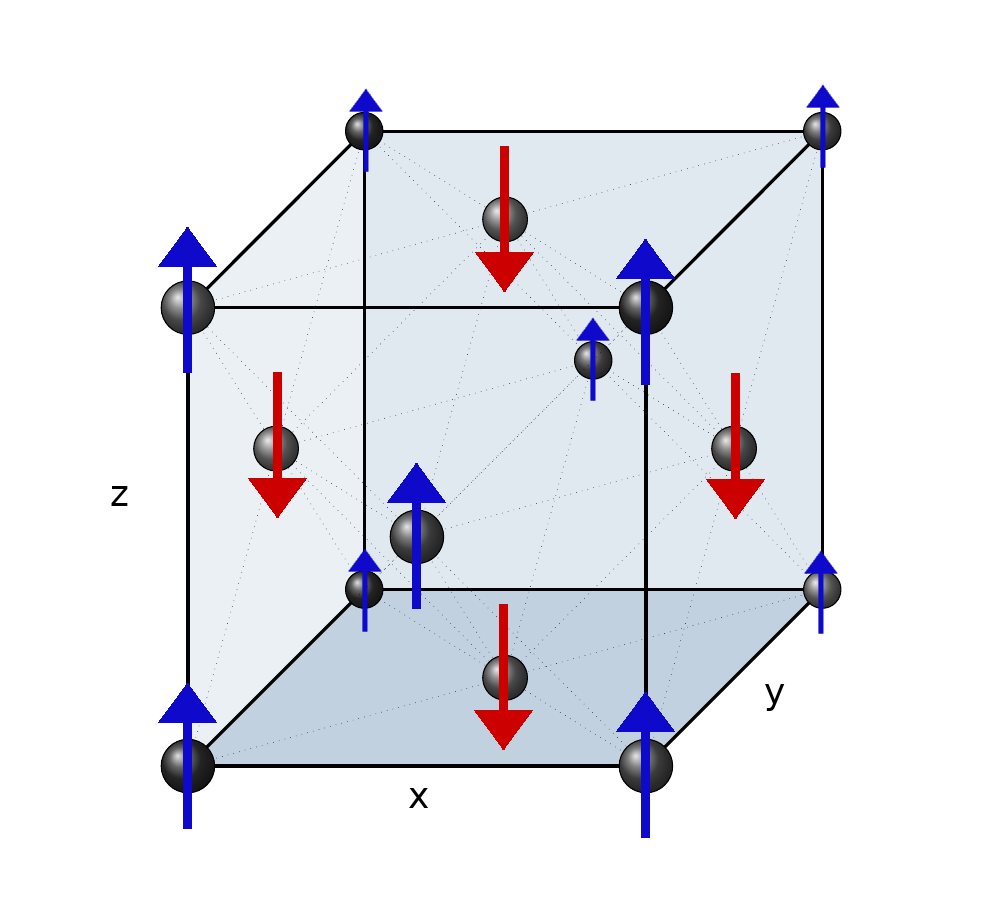
\includegraphics[width=.7\linewidth]{chapters/potentials_fe_pd_ru/images/fe-austenitic-mag.png} 
  \caption{Magnetic alignment along the z-axis, antiferromagnetic Fe fcc}  
  \label{fig:ironfccantiferromagnetic}
\end{figure}

The atoms in the (0,1,0) plane are majority spin-up electrons, along the z-axis, and those in the (0,2,0) plane are spin-down, along the z-axis (fig. \ref{fig:ironfccantiferromagnetic}).  Following the relaxation calculation, all the atoms were in their standard \acrshort{fcc} positions, and the magnetic moment for each atom was 1.4901 \gls{bohrmagneton} and -1.4901 \gls{bohrmagneton} for the spin up and down respectively.  





\FloatBarrier
\subsection[Elastic Constants]{Calculation of Elastic Constants}
\label{section:resultselastic}

The planewave cutoff and k-points were converged to within the required parameters for energy and force but it is known that, in general, \acrshort{lda} and \acrshort{gga} pseudopotentials under and over estimate the lattice parameters.  The bulk modulus and elastic constants were calculated for \acrshort{fcc} Aluminium and \acrshort{bcc} Iron in order to compare to experimental values.

A summary of the main data points is given here for \acrshort{fcc} Al, \acrshort{bcc} Fe, \acrshort{fcc} Pd and \acrshort{fcc} Fe, and the first three listed are compared to experimental data.  A full details of the calculated properties including plots are included in appendix \ref{chapter:dftcalculatedproperties}.

\subsubsection{FCC Aluminium}

The parameters used for the Al calculations were arrived at earlier using the convergence code.  The remainder of the parameters are either default settings, or were selected following trial and error (for example, reducing the mixing beta to help achieve convergence).  These settings are given in table \ref{table:alfccdftsettings}.

The results in table \ref{table:alfccexperimentaldft} show a good agreement between the experimental values for Al and the calculated values.  The lattice parameter is a particularly good fit, being within 1\% of the experimental value.  The shear modulus does not match as well, but is within 20\% of the experimental value.  The \acrshort{rss} measurement of fit between the values was $2.54 \times 10^2$.


\FloatBarrier
\subsubsection{BCC Iron}

The equation of state and elastic constants were calculated for \acrshort{bcc} Fe, with no-spin and collinear spin.  The settings used for the calculations are given in table \ref{table:febccdftsettings}. 


The non-magnetic Iron calculation was particularly poor.  Although the lattice parameter was within 5\% of the experimental value, the structure was unstable and had negative values for both the Young's modulus and shear modulus (table \ref{table:febccexperimentaldft}).  The \acrshort{rss} measurement of fit between the values for the was $2.01 \times 10^5$.

With collinear spin enabled, the structure is stable.  The lattice parameter is still slightly under the experimental, but is now within almost 2\% of the value.  The bulk modulus predicted by fitting the Birch-Murnaghan equation of state is more than 40\% the experimental value, but the Reuss and Voigt values derived from the calculated elastic constants are just 20\% difference to the experimental value.  The latter two values are calculated using the elastic constants, rather than the equation of state.  This highlights the importance of using collinear spin calculations, despite the cost in computing time.  The \acrshort{rss} measurement of fit between the values was $1.09 \times 10^4$ giving an improvement of at least one magnitude.




\FloatBarrier
\subsubsection{FCC Iron}
\label{section:fccferesults}

The gamma phase of pure iron does not exist for experimental measurements to be made, and the results here will be used to fit the FCC iron potential in chapter \ref{chap:resultsfitting}.  The settings used for the calculations are given in table \ref{table:fefccdftsettings}. 

The structure is stable under the orthorhombic stability conditions given in section \ref{section:stabilityconditions}.  Whilst there are no experimental measurements to check against, the values are sane when compared to the other calculations performed here (table \ref{table:fefccexperimentaldft}).  The $C_{44}$, $C_{55}$ and $C_{66}$ values are slightly large when compared with those for \acrshort{bcc}, but further \acrshort{dft} calculations would need to be performed to investigate this.  

\begin{table}[ht]
\renewcommand{\arraystretch}{1.2}
\begin{tabular}{lccc}
\hline\hline
Property & \multicolumn{3}{c}{Value used in potential fitting} \\
\hline\hline
Element & \multicolumn{3}{c}{Fe}\\
Structure             & \multicolumn{3}{c}{Face Centered Cubic}\\
$a_0$                 & \multicolumn{3}{c}{3.59 Angstrom}\\
Nearest Neighbour     & \multicolumn{3}{c}{1.85 Angstrom}\\
Basis vectors         & $\begin{bmatrix} 0.96 & 0.0 & 0.0 \\ 0.0 & 1.00 & 0.0 \\ 0.0 & 0.0 & 0.96  \end{bmatrix}$ \\
$E_{coh}$             & \multicolumn{3}{c}{-4.32 eV}   \\
$B_0$ (GPA)           & \multicolumn{3}{c}{226.1}   \\
$E$ (GPA)             & \multicolumn{3}{c}{356.8}   \\
$G$ (GPA)             & \multicolumn{3}{c}{144.8}   \\
Poisson Ratio $\eta$  & \multicolumn{3}{c}{0.23}   \\
Elastic Constants     & $\begin{bmatrix} 364.6 & 141.6 & 233.8 & 0 & 0 & 0 \\ 141.6 & 298.7 & 130.4 & 0 & 0 & 0 \\ 233.8 & 130.4 & 364.6 & 0 & 0 & 0 \\ 0 & 0 & 0 & 186.3 & 0 & 0 \\ 0 & 0 & 0 & 0 & 266.8 & 0 \\ 0 & 0 & 0 & 0 & 0 & 186.3 \end{bmatrix}$ \\
\hline\hline
\end{tabular}
\caption{Fe input parameters for fitting}
\label{table:feinputparameters}
\end{table}








\FloatBarrier
\subsubsection{FCC Palladium}

The equation of state and elastic constants were calculated for \acrshort{fcc} Pd with no-spin.  The settings used for the calculations are given in table \ref{table:pdfccdftsettings}. 

There is a good agreement between the computed and experimental values for Pd, without the need to move from non-spin to collinear spin calculations (table \ref{table:pdexperimentaldft}).  However, in the alloy calculations the  presence of Fe will dictate the necessity for collinear spin.  The \acrshort{rss} measurement of fit between the values was $4.12 \times 10^3$.

\begin{table}[ht]
\renewcommand{\arraystretch}{1.2}
\begin{tabular}{lccc}
\hline\hline
Property & \multicolumn{3}{c}{Value used in potential fitting} \\
\hline\hline
Element & \multicolumn{3}{c}{PD}\\
Structure             & \multicolumn{3}{c}{Face Centered Cubic}\\
$a_0$                 & \multicolumn{3}{c}{3.925 Angstrom \cite{webelementspd}}\\
Nearest Neighbour     & \multicolumn{3}{c}{ Angstrom \cite{webelementspd}}\\
Basis vectors         & $\begin{bmatrix} 1.0 & 0.0 & 0.0 \\ 0.0 & 1.0 & 0.0 \\ 0.0 & 0.0 & 1.0  \end{bmatrix}$ \\
$E_{coh}$             & \multicolumn{3}{c}{3.91 eV \cite{semiempiricalpots}}   \\
$B_0$                 & \multicolumn{3}{c}{184.4 GPA \cite{semiempiricalpots}}   \\
Elastic Constants     & $\begin{bmatrix} 218.5 & 151.4 & 151.4 & 0 & 0 & 0 \\ 151.4 & 218.5 & 151.4 & 0 & 0 & 0 \\ 151.4 & 151.4 & 218.5 & 0 & 0 & 0 \\ 0 & 0 & 0 & 80.3 & 0 & 0 \\ 0 & 0 & 0 & 0 & 80.3 & 0 \\ 0 & 0 & 0 & 0 & 0 & 80.3 \end{bmatrix}$ \\
\hline\hline
\end{tabular}
\caption{Pd input parameters for fitting}
\label{table:pdinputparameters}
\end{table}





\FloatBarrier
\subsubsection{FCC Ruthenium}
\label{section:fccferesults}


Ruthenium at standard conditions exists as \acrlong{hcp}, but as this work is focused on \acrshort{fcc} steel doped with \acrshort{pgm}s, the properties are computed for \acrshort{fcc} Ruthenium.  The settings used for the calculations are given in table \ref{table:rufccdftsettings}. 



\begin{table}[ht]
\renewcommand{\arraystretch}{1.2}
\begin{tabular}{lccc}
\hline\hline
Property & \multicolumn{3}{c}{Value used in potential fitting} \\
\hline\hline
Element & \multicolumn{3}{c}{RU}\\
Structure             & \multicolumn{3}{c}{Face Centered Cubic}\\
$a_0$                 & \multicolumn{3}{c}{3.809 Angstrom \cite{webelementspd}}\\
Nearest Neighbour     & \multicolumn{3}{c}{ Angstrom \cite{webelementspd}}\\
Basis vectors         & $\begin{bmatrix} 1.0 & 0.0 & 0.0 \\ 0.0 & 1.0 & 0.0 \\ 0.0 & 0.0 & 1.0  \end{bmatrix}$ \\
$E_{coh}$             & \multicolumn{3}{c}{6.624 eV \cite{semiempiricalpots}}   \\
$B_0$                 & \multicolumn{3}{c}{307.8 GPA \cite{semiempiricalpots}}   \\
Elastic Constants     & $\begin{bmatrix} 471.5 & 219.1 & 219.1 & 0 & 0 & 0 \\ 219.1 & 471.5 & 219.1 & 0 & 0 & 0 \\ 219.1 & 219.1 & 471.5 & 0 & 0 & 0 \\ 0 & 0 & 0 & 245.0 & 0 & 0 \\ 0 & 0 & 0 & 0 & 245.0 & 0 \\ 0 & 0 & 0 & 0 & 0 & 245.0 \end{bmatrix}$ \\
\hline\hline
\end{tabular}
\caption{Pd input parameters for fitting}
\label{table:ruinputparameters}
\end{table}




\subsection{Calibrating the Cohesive Energies}

\acrlong{dft} solves the Kohn-Sham equations for an infinite repeating lattice, and at first it doesn't seem applicable to single atoms or molecules that are not part of much larger lattice.  There are settings that may be used to compute the energy of an isolated atom and these are discussed on the Quantum Espresso forum\cite{qeforum} and Materials Square\cite{materialssquaresingleatom}. 

The settings of note used in these calculations were a configuration of just 1 isolated atom in a large cubic cell (20+ Bohr).  The computations were all nspin = 2 to ensure the electrons are computed spin up and down.  The assume\_isolated setting is given the makov-payne setting, as the system is a cube.

It was important to reduce the number of processor cores as too many would cause matrix decomposition errors for a low number of atoms, causing Quantum Espresso to crash.  An option to leverage more cores was to split the calculation into pools using the -npool input flag for PWscf, but this was not necessary for this set of calculations.


The isolated and relaxed energy values were computed and from these values the cohesive energies were calculated (figure \ref{fig:isolatedatoms} and table \ref{table:calculatedcohesiveenergies}).  In doing so, it became apparent that there were errors of up to 12\% between the known values and those computed with \acrshort{dft}.

\begin{figure}[h]
\begin{center}
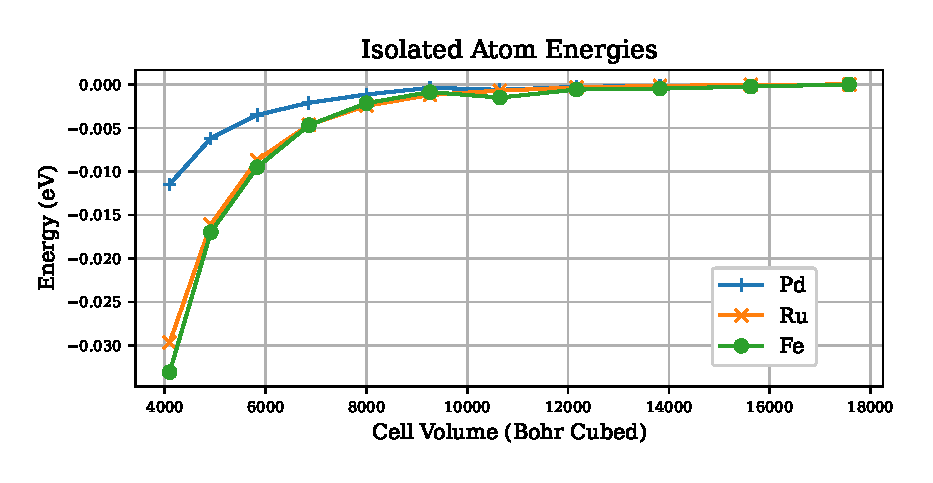
\includegraphics[width=0.5\linewidth]{chapters/potentials_fe_pd_ru/isolated/isolated_63.eps}
\caption{Isolated atom energies as cell size increase}
\label{fig:isolatedatoms}
\end{center}
\end{figure}

An offset was needed to convert from the \acrshort{dft} energies to \enquote{real} energies that could be used to derive a potential.

\begin{table}[h]
\begin{center}
\begin{tabular}{c c c c c}
\hline\hline
Element & Structure & Isolated Energy (Ry) & Relaxed Energy (Ry) & Cohesive Energy (eV) \\
\hline\hline
Fe      & BCC       & -4474.99115          & -4479.83524         & 4.84 (exp. 4.32)\\
Fe      & FCC       & -4474.99115          & -4479.78095         & 4.79 \\
Pd      & FCC       & -6962.47261          & -6966.52234         & 4.05 (exp. 3.91)\\
Ru      & HCP       & -5866.39894          & -5873.22666         & 6.83 (exp. 6.74)\\
Ru      & FCC       & -5866.39894          & -5873.11029         & 6.71 \\
\hline\hline
\end{tabular}
\end{center}
\caption{\acrshort{dft} calculated energies per atom}
\label{table:calculatedcohesiveenergies}
\end{table}

Two offsets were computed and these depend upon the settings used in the calculation (table \ref{table:calculatedoffset}).  Specifically, they depend on whether 9x9x9 k-points are used, in the case of the 32 atom calculations, or the gamma point is used (128, 129 and 256 atoms).

\begin{table}[h]
\begin{center}
\begin{tabular}{c c c c c}
\hline\hline
Element & Reference Structure & Energy (Ry) (9x9x9) & Energy (Ry) (Gamma) & Cohesive (eV)\\
\hline\hline
Fe      & BCC  & -329.2618197  & -84290.00709480 & -4.316 \\
Pd      & FCC  & -512.0299524  & -131079.09207327 & -3.91 \\
Ru      & HCP  & -431.6742014  & -110507.45936537 & -6.74 \\
\hline\hline
\end{tabular}
\end{center}
\caption{Relaxed energies for 32 atoms, using 9x9x9 k-points, and 256 atoms, using the gamma point.  These were used with the known cohesive energy to compute the offset energy.}
\label{table:calculatedoffset}
\end{table}





\subsection[DFT Reference Database]{Compiling a DFT Reference Database}


A database of configurations generated by \acrshort{dft} was compiled for Iron, Palladium, Ruthenium with alloys of Iron-Palladium and Iron-Ruthenium.  The potentials are derived for \acrshort{fcc} Iron and so these configurations were also \acrshort{fcc}.

The QEEOS code was used to compute the bulk properties and in doing so it created PWscf input files and processed the output files.  These output files are saved but the program and are as valid to use in the reference database as any.  In total the database has over 600 configurations for Fe-Pd and almost 600 for Fe-Ru.  

\begin{figure}
\begin{subfigure}{.32\textwidth}
  \centering
  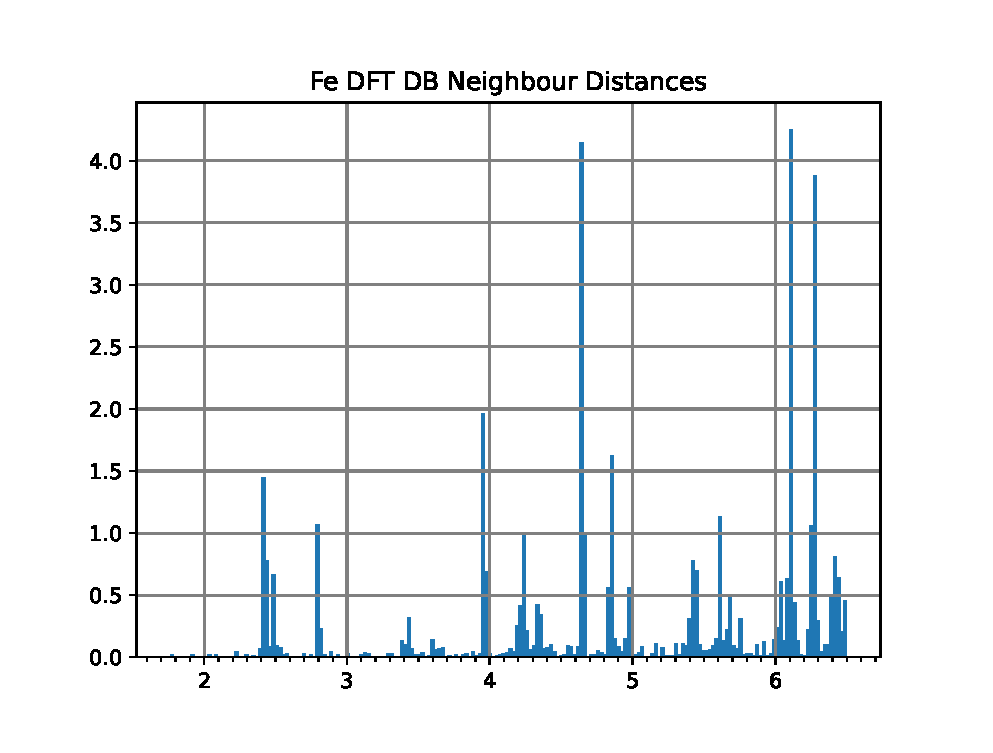
\includegraphics[width=.94\linewidth]{chapters/potentials_fe_pd_ru/neighbour_distances/db_fe_neighbours.eps}  
  \caption{Single atom, 256 atoms in total}
  \label{fig:sub-first}
\end{subfigure}
\begin{subfigure}{.32\textwidth}
  \centering
  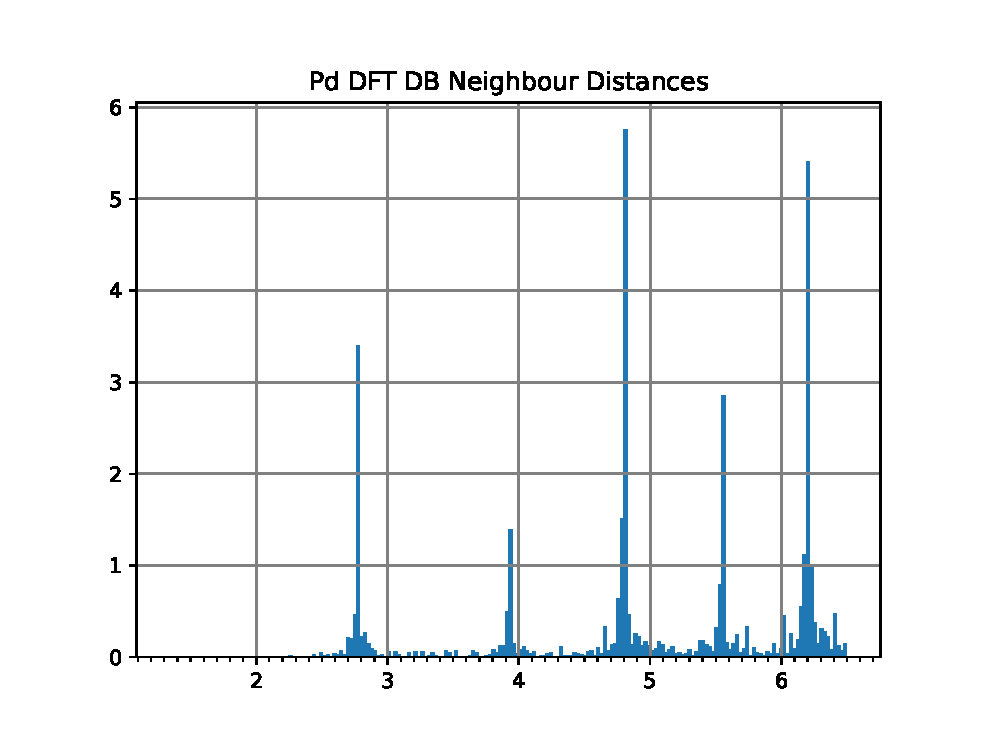
\includegraphics[width=.94\linewidth]{chapters/potentials_fe_pd_ru/neighbour_distances/db_pd_neighbours.eps}  
  \caption{Multiple atoms, 256 atoms in total}
  \label{fig:sub-first}
\end{subfigure}
\begin{subfigure}{.32\textwidth}
  \centering
  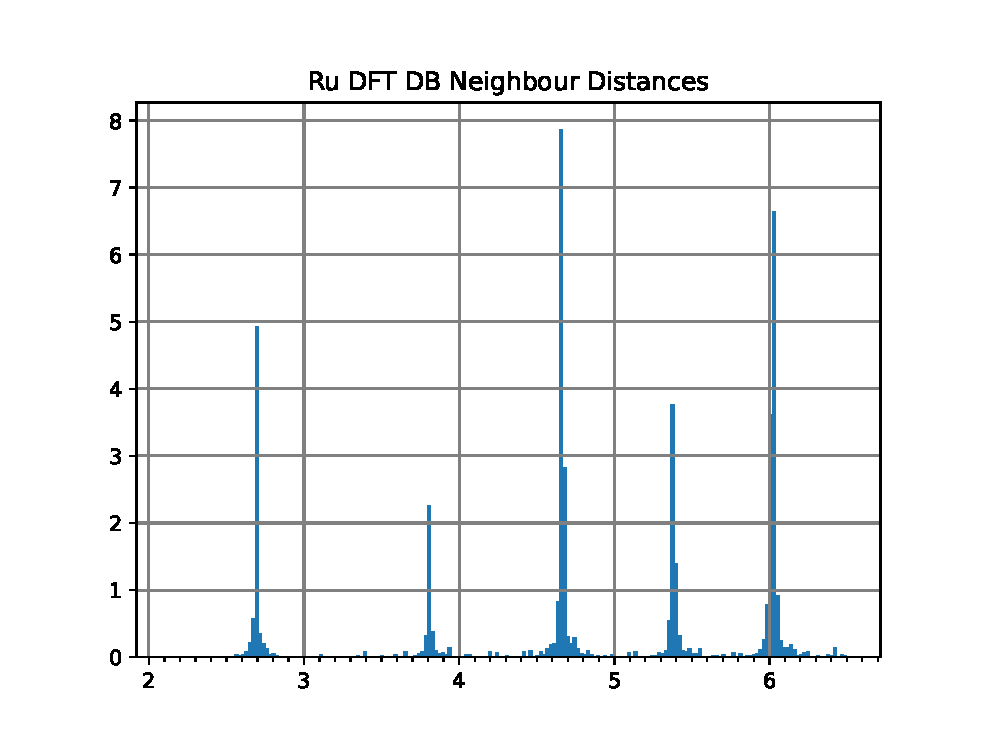
\includegraphics[width=.94\linewidth]{chapters/potentials_fe_pd_ru/neighbour_distances/db_ru_neighbours.eps}  
  \caption{Multiple atoms, 256 atoms in total}
  \label{fig:sub-first}
\end{subfigure}
\begin{subfigure}{.32\textwidth}
  \centering
  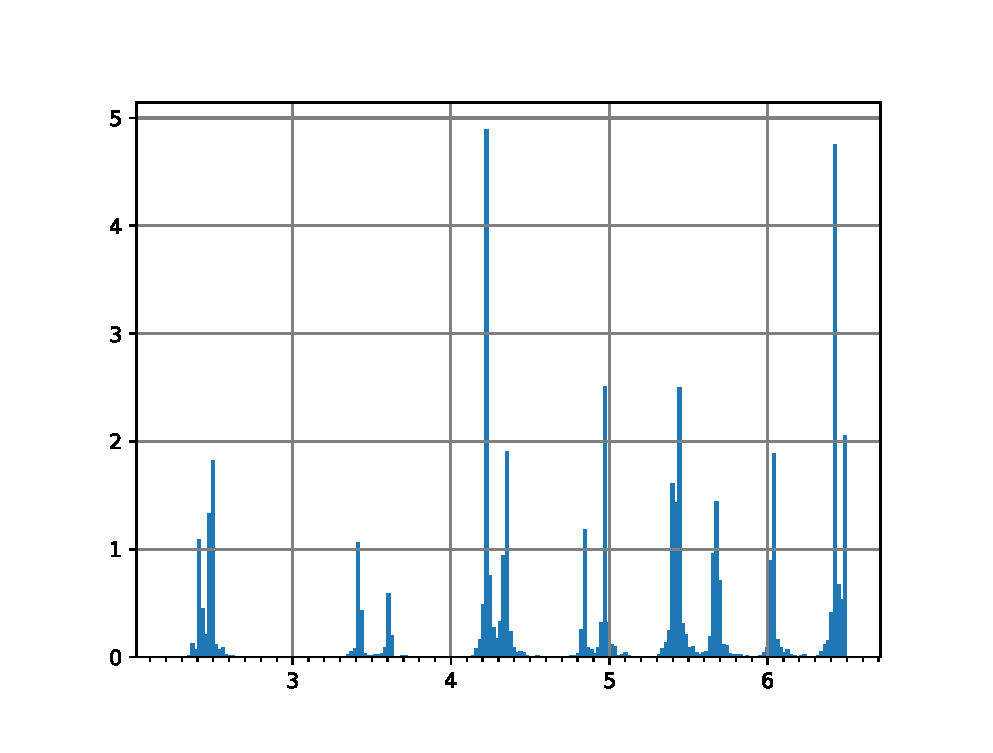
\includegraphics[width=.94\linewidth]{chapters/potentials_fe_pd_ru/neighbour_distances/db_fepd_neighbours.eps}  
  \caption{Multiple atoms, 256 atoms in total}
  \label{fig:sub-first}
\end{subfigure}
\begin{subfigure}{.32\textwidth}
  \centering
  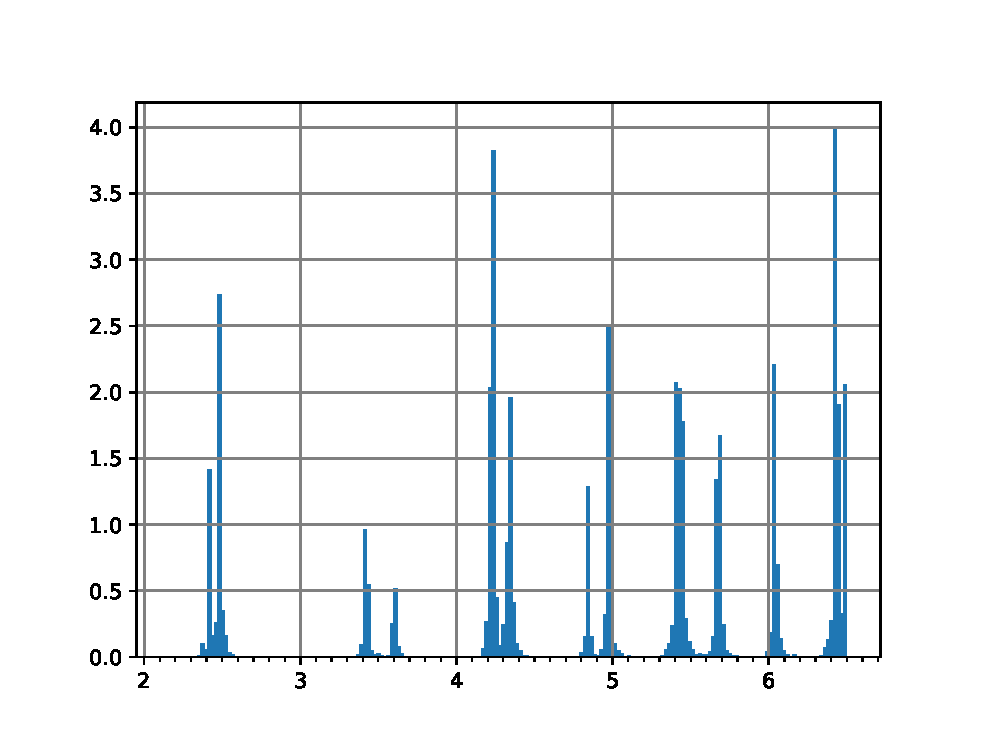
\includegraphics[width=.94\linewidth]{chapters/potentials_fe_pd_ru/neighbour_distances/db_feru_neighbours.eps}  
  \caption{Multiple atoms, 256 atoms in total}
  \label{fig:sub-first}
\end{subfigure}
\label{fig:dbneighbourseparations}
\end{figure}

The distribution of atom separations was measured across the database and these are plotted in figure \ref{fig:dbneighbourseparations}.  The full set is available to download from https://github.com/BenPalmer1983/fepd\_feru\_potential.

All the configurations in this work are \acrshort{fcc} structure crystals.  The QEEOS program (section \ref{section:qeeospyprog} and \ref{code:qeeos}) was used to compute the relaxed lattice parameter and primitive cell basis vector.

This program also automated the computation of equation of state, bulk modulus and elastic constants.  A 32 atom supercell was used for each pure element where the bulk properties were computed.  Ideally a large supercell or a larger number of k-points would have been used but throughout this work the number of processor cores per node ranged from 20-72 and this along with time constraints limits complexity of the calculations.

The data output from the QEEOS code forms a part of the reference database that is discussed in chapter \ref{chap:resultsdftdb}.





\subsection{Pure Element Defects}

The potentials are created to apply to \acrshort{fcc} Iron, Palladium, Ruthenium and alloys of Fe-Pd and Fe-Ru.  The configuration database will include several defects:

\begin{itemize}
\item octahedral interstitial
\item tetrahedral interstitial
\item 100, 110 and 111 interstitials
\item crowdion
\item a vacancy
\end{itemize}

The configurations for these defects were estimated using the perfect crystal positions of 2x2x2 supercells containing 32 atoms.  The defect or vacancy was applied, in some cases changing the total number of atoms, and the defect position was estimated.

A number of calculations, and the chance of a successful convergence in both the electronic state \acrshort{scf} calculation and relaxation calculation, were very sensitive on the input parameters.  Aluminium was not as sensitive and was used to relax the starting configuration.  This was then used as the starting point for either Fe, Pd or Ru.

Due to the periodic nature of these calculations, having only 32 atoms was not ideal as each defect cell would be very close to another.  Unfortunately, as stated a number of times, it was a constraint that was needed to be able to complete the work in a reasonable amount of time.

\FloatBarrier
\subsection{Alloy Atom Positions for Pd and Ru}

The stainless steel being studied is to be doped with 1\% or less of a \acrlong{pgm}.  Ideally a super cell with at least 256 atoms (4x4x4 primitive \acrshort{fcc} cells) would be used for all calculations, but due to the complexity of the calculations the majority were 2x2x2 super cells containing just 32 atoms.

\begin{figure}[htb]
\begin{subfigure}{.42\textwidth}
  \centering
  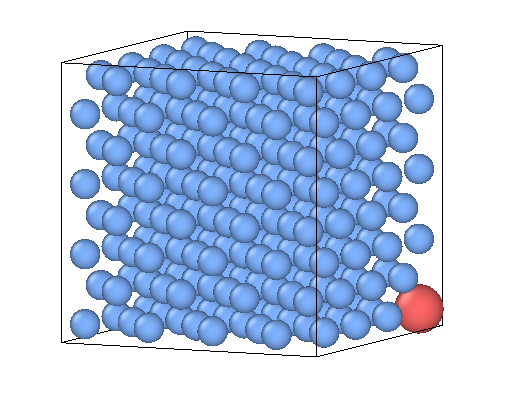
\includegraphics[width=.94\linewidth]{chapters/potentials_fe_pd_ru/slabs/bulk01.png}  
  \caption{Single atom, 256 atoms in total}
  \label{fig:sub-first}
\end{subfigure}
\begin{subfigure}{.42\textwidth}
  \centering
  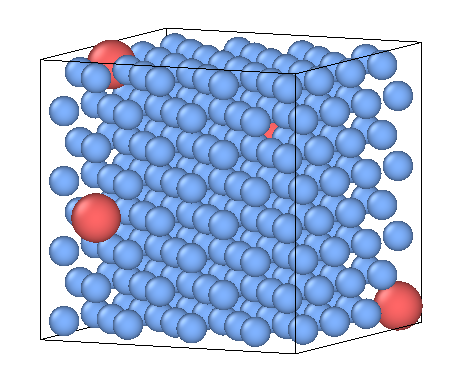
\includegraphics[width=.94\linewidth]{chapters/potentials_fe_pd_ru/slabs/bulk02.png}  
  \caption{Multiple atoms, 256 atoms in total}
  \label{fig:sub-first}
\end{subfigure}
\label{fig:binaryalloyconfigurationsbulk}
\end{figure}

Most of the configurations were prepared using the relaxed \acrshort{fct} structure computed for Fe.  One or more iron atoms were then replaced with either Pd or Ru.  The majority of calculations were carried out using the 32 atom configurations.  The larger 256 atom calculations were better suited to represent the low percentage of \acrshort{pgm} but were only computed using the gamma k-point (figure \ref{fig:binaryalloyconfigurationsbulk}).  This was another compromise in order to complete the calculations in time.



\subsection{Configurations with Randomised Positions}

Many of the atom configurations generated up to this point are symmetric and, whilst they have a variety of energies and stresses to use for fitting, the forces on the atoms are almost balanced and are small or none.  A large set of configurations with positions perturbed slightly from the exact lattice position are created.

Rather than use a linear random distribution a Gaussian distribution is used.  Some atoms had a larger perturbation but the majority are be slightly closer to the exact position, as would be expected with this type of distribution.  The maximum amount of perturbation was selected randomly between a minimum and maximum value.  

\begin{figure}[h]
\begin{center}
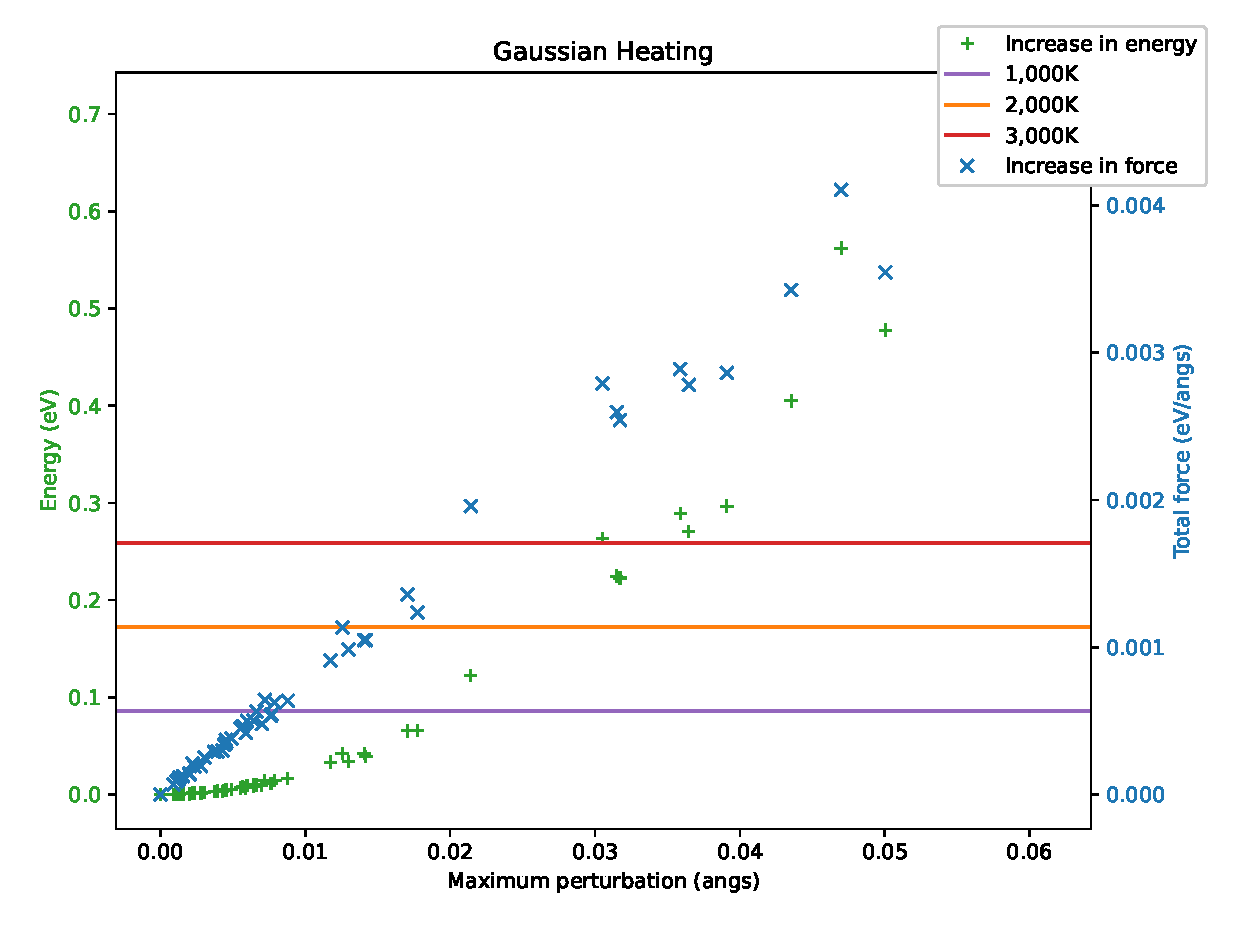
\includegraphics[scale=0.45]{chapters/potentials_fe_pd_ru/pwheat/al/alheat.eps}
\caption{Effect of randomly perturbing atom locations}
\label{fig:pwheatal}
\end{center}
\end{figure}

As the amount at which the atoms are perturbed increases, the energy and total force between the atoms increases.  If the disturbance increases too much, it will likely be useless for our needs as it would be beyond the temperatures relevant to this work, and it may also cause the \acrshort{scf} calculations to fail.

In the case of the alloy configurations, the randomised positions were loaded into the files.  In all cases convergence failed.  As perturbed atom positions had already been computed for Fe a new set of input files were created holding the Fe atoms in their perfect locations.  The added Pd and Ru atoms were then perturbed slightly from their perfect position within the lattice in order to compute forces and energies at slightly different positions.


\FloatBarrier
\subsection{Surface Energy Calculations}

One key aspect of this work is to determine whether or not either Pd or Ru are depleted from the surface at grain boundaries under irradiation.  With this in mind, the surface energies for the pure elements were calculated by creating a slab of atoms with an open surface on each side.

\begin{figure}[htb]
\begin{subfigure}{.32\textwidth}
  \centering
  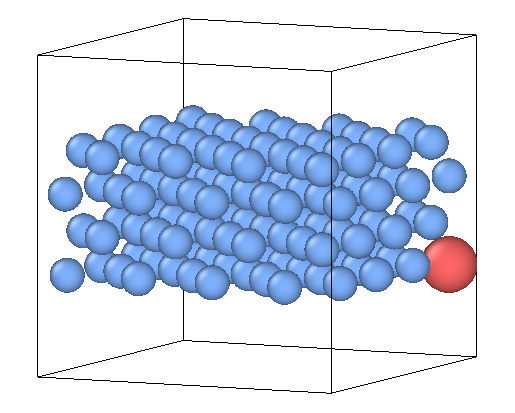
\includegraphics[width=.94\linewidth]{chapters/potentials_fe_pd_ru/slabs/slab01.png}  
  \caption{Single atom in the surface layer, 128 atoms in total}
  \label{fig:sub-first}
\end{subfigure}
\begin{subfigure}{.32\textwidth}
  \centering
  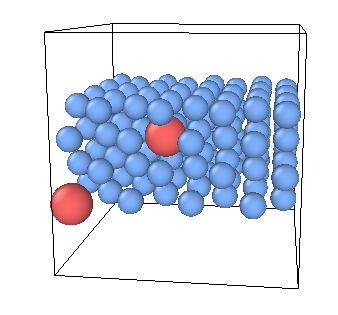
\includegraphics[width=.94\linewidth]{chapters/potentials_fe_pd_ru/slabs/slab02.png}  
  \caption{Single atom in bulk of slab, single atom in surface layer, 128 atoms in total}
  \label{fig:sub-first}
\end{subfigure}
\begin{subfigure}{.32\textwidth}
  \centering
  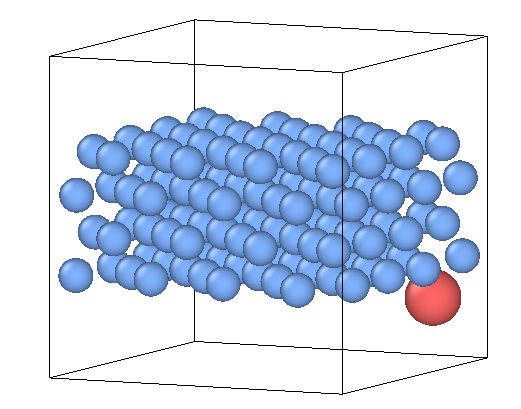
\includegraphics[width=.94\linewidth]{chapters/potentials_fe_pd_ru/slabs/slab03.png}  
  \caption{Single atom on the surface, 129 atoms in total}
  \label{fig:sub-first}
\end{subfigure}
\caption{A sample of configurations used for binary alloy \acrshort{dft} calculations for Fe-Pd and Fe-Ru.}
\label{fig:binaryalloyconfigurationsslab}
\end{figure}

A set of 32 atom configurations are used where the separation between the two facing surfaces is varied.  Several more 128 atom configurations are also prepared for the three pure elements.  To investigate the effect of a small addition of either Ru or Pd in the alloy a slab of Fe was prepared with Ru or Pd either within the slab, at the surface or on the surface (figure \ref{fig:binaryalloyconfigurationsslab}).  These examples were then added into the reference database used to fit the binary potentials.



\FloatBarrier
\subsection{Defects in Fe-Pd and Fe-Ru Alloys}

Attempts were made to compute simple defects in the alloy but the majority failed to converge, either in the electronic structure \acrshort{scf} iteration or a failure to relax geometrically that then lead to a \acrshort{scf} failure.  Rather than focus too much on this, more time was spent investigating Ru and Pd in a slab of Fe where the calculations were more successful.















